\documentclass[convert={density=300,size=1080x800,outext=.png}]{standalone}
\usepackage{tkz-graph}
\usetikzlibrary{arrows,positioning,shapes,shapes.multipart,patterns,mindmap,shadows}
\usepackage{xcolor}
\usepackage{helvet}
\renewcommand{\familydefault}{\sfdefault}


\begin{document}

\footnotesize
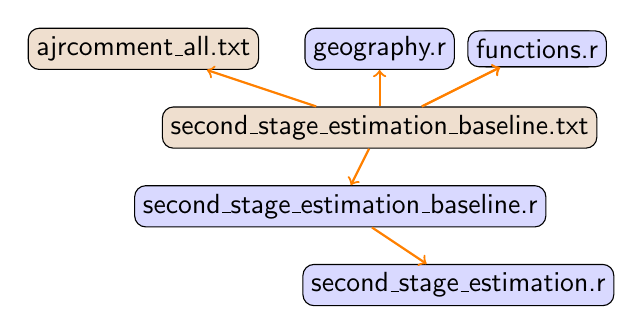
\begin{tikzpicture}[every node/.style={
    rectangle,
    rounded corners,
    inner sep=3pt,
    draw,
    fill=brown!25
}]
    \node (ajrcomment_all_txt) [shift={(2, 0)}]
    {
        ajrcomment\_all.txt
    };



    \node (geography_r) [fill=blue!15, shift={(5, 0)}]
    {
        geography.r
    };
    \node (baseline_r) [fill=blue!15, shift={(7, 0)}]
    {
        baseline.r
    };
    \node (functions_r) [fill=blue!15, shift={(7, 0)}]
    {
        functions.r
    };



    \node (second_stage_estimation_baseline_txt) [shift={(5, -1)}]
    {
        second\_stage\_estimation\_baseline.txt
    };



    \node (second_stage_estimation_baseline_r) [fill=blue!15, shift={(4.5, -2)}]
    {
        second\_stage\_estimation\_baseline.r
    };


    \node (second_stage_estimation_r) [fill=blue!15, shift={(6, -3)}]
    {
        second\_stage\_estimation.r
    };




    \draw[->, orange, thick] (second_stage_estimation_baseline_txt) to (second_stage_estimation_baseline_r);
    \draw[->, orange, thick] (second_stage_estimation_baseline_txt) to (geography_r);
    \draw[->, orange, thick] (second_stage_estimation_baseline_txt) to (ajrcomment_all_txt);
    \draw[->, orange, thick] (second_stage_estimation_baseline_txt) to (baseline_r);
    \draw[->, orange, thick] (second_stage_estimation_baseline_txt) to (functions_r);
    \draw[->, orange, thick] (second_stage_estimation_baseline_r) to (second_stage_estimation_r);


\end{tikzpicture}

\end{document}

